
\chapter{Øyesporing}

Øyesporing refereres ofte til teknikken brukt til å fange og måle øyebevegelser \cite{Calibration}. Målet med dette kapittelet er å gi en beskrivelse av hvordan øyesporing fungerer og enheten som brukes i denne avhandlingen - samt en forklaring av viktige konsepter.


\section{Hvordan fungerer øyet?}

Å forklare hvordan øyet fungerer i detalj er utenfor denne rapportens omfang. Det vil derfor kun gis en høynivå forklaring av hvordan det fungerer for å kunne forstå det som er nødvendig i henhold til rapporten. 

\subsection{Synsfelt}

I en artikkel skrevet av Tobii \cite{Calibration} sammenlignes øyet med et fotoapparat på grunn av dens mange likhetstrekk. Når lys treffer et objekt reflekteres dette, det reflekterte lyset reiser så gjennom en linse og ender opp i øyet. Linsen prosjekterer lyset den mottar på en lyssensitiv overflate. Denne overflatens oppførsel er også det som skiller øyet fra fotoapparatet. For i motsetning til et kamera er ikke overflaten like sensitiv overalt i øyet.  Dette gjør at menneske kan tilpasse synet etter hvor mye lys som er tilgjengelig. En bieffekt er at det også resulterer i at menneske kun kan se klart i begrensede områder av synsfeltet. Figur \ref{fig:visueltArea} illustrerer hvordan synsfeltet hos menneske er delt inn etter klarhet. (F) representerer det foveale området. Dette er området man fokuserer på og oppfatter klarest. Det er hovedsaklig fra dette området visuell data hentes fra . (Pf) viser det parafovela omårdet, som kjennetegnes ved at uskarpheten øker til man kommer til det perifere området. (P) Det perifere området, også kjent som sidesynet, fungerer kun bra til å fange opp bevegelser og kontraster.

\begin{figure}[ht!]
\centering
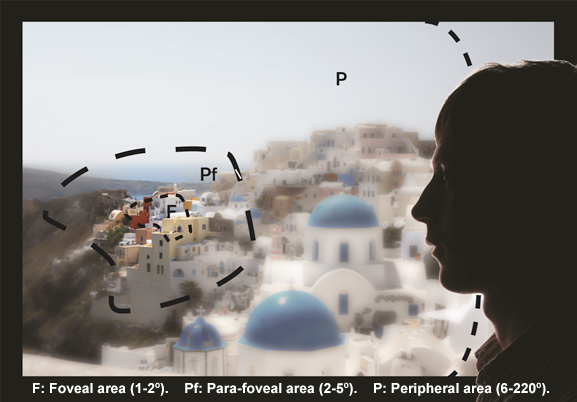
\includegraphics[width=65mm]{fovealArea}
\caption{Bilde/Illustrasjon av menneskelige synsfelt \cite{VisualImage}}
\label{fig:visueltArea}
\end{figure}

\subsection{Fikseringer og sakkader}

Det foveale området er som nevnt det området det registreres mest visuell data. Området står derimot for mindre 8 prosent av synsfeltet. Dette gjør at for å kunne innhente informasjon av interesse fra andre deler av synsfeltet må det flyttes inn i  det foveale området. For å gjøre det brukes øyeoperasjoner kalt fikseringer og sakkader. Fikseringer er pauser fra bevegelsen på et område, sakkader er hurtige bevegelser mellom fikseringene \cite{Calibration}.


\section{Hvordan fungerer øyesporing?}

Øyesporing er som tidligere nevnt teknikken brukt til å fange og måle øyebevegelser.
Det finnes derimot flere fremgangsmåter. I denne oppgaven vil det brukes en ikke-forstyrrende øyestyringsenhet. Dette gjør at brukeren i prinsippet ikke skal legge merke til enheten. For denne typen øyesporing er det mest vanlig å bruke en teknikk som heter Pupil Centre Cornea Reflection (\gls{PCCR}) \cite{Calibration}. Teknikken fungerer ved at en lyskilde belyser øyet for at refleksjonene skal bli klare og synlige. Et kamera tar deretter bilde av refleksjonene fra øyet. Bildet blir så brukt til å identifisere lysets refleksjon på hornhinnen og pupillen. Når en vet vinkelen mellom hornhinnen og pupillen er det mulig å regne ut en vektor. Vektoren sammen med andre geometriske egenskaper ved refleksjonene gjør det mulig å kalkulere ut blikkretningen(Der brukeren ser) \cite{Calibration}.


\subsection{Utfordringer}

En utfordring ved øyesporing er blunking. Blunking er et er en kortvarig sammentrekning av øyelokket, noe som gjør at øyet ikke vil gi refleksjon som kamera kan fange, og derfor ikke ha koordinater på hvor brukeren ser. Dette løses under analysen. Ved at og bruke koordinatene og øyets hurtighet før øyelokkene trakk seg sammen kan man ekstrapolere seg fram til en tilnærmet korrekt fiksering. 

\section{Tobii PCEye Go}

I denne rapporten brukes øyesporingsenheten Tobii PCEye GO, som vist i figur \ref{fig:tobiiPc}. Enheten kommer separat og kobles til datamaskinen via USB. Dette er som tidligere nevnt et ikke-forstyrrende apparat. Et eksempel på det motsatte ville vært et par briller som ble brukt til å spore øyebevegelser. 



\begin{figure}[ht!]
\centering
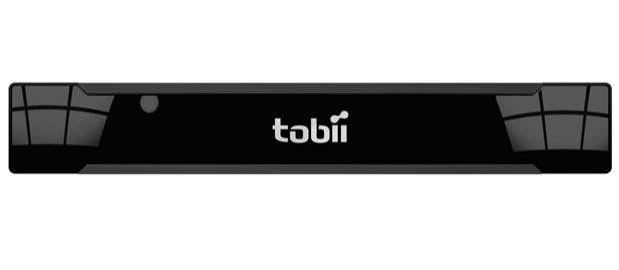
\includegraphics[width=50mm]{TobiiEyeGo}
\caption{Bilde av øyestyringsenheten Tobii PCEye Go}
\label{fig:tobiiPc}
\end{figure}


\subsection{Tobii blikkprogramvare}
\label{subsec:blikk}

Sammen med Tobii PCeye go følger det med programvare for å kontrollere applikasjoner som bruker sporingsenheten. Den består av følgende komponenter: 

\begin{itemize}
\item [Blikk interaksjonsserver] en sentral HUB som tilbyr klient applikasjoner øyesporingsdata. 
\item [Blikk interaksjons innstillinger] Et kontrollpanel for interaksjons innstillinger og oppgaver relatert til øyesporing
\item [Windows Kontroll] Tilbyr blikk interaksjon for standard Windows applikasjoner, ergo vanlige applikasjoner som ikke er laget for øyesporings interaksjon.
\end{itemize}

I denne rapporten vil kun førstnevnte være relevant. Ettersom applikasjonen er spesialisert til blikk interaksjon og ikke er en standard Windows applikasjon.

\subsection{Blikk Interaksjonsserver}

Blikk interaksjons-serveren er som nevnt i seksjon \ref{subsec:blikk} en HUB for programvaren, eller kjernen. Hovedformålet til denne komponenten er å samhandle med Øye-sporingsenheten og tilby interaksjonsfunksjonalitet for å kontrollere Windows baserte applikasjoner som vil bruke sporingsdata. I tilegg er det denne komponenten som tar seg av kalibrering, sporingsstatus - samt bruker og applikasjons innstillinger.

\subsection{Tobii Eye Control API }

Figur \ref{fig:overview} viser hvordan blikk interaksjonsserveren eksponerer funksjonalitet til en klient-applikasjon gjennom et APIet, som er kalt Tec API. For å ta i bruk TecAPIet tilbys to aksess punkter. Et gjennom .NET plattformen kalt TecClient og et for C dynamisk link library kalt MPACI.  Den praktiske betydningen, er at man kun kan bruke APIet ved å skrive i C eller .NET teknologier. I denne rapporten vil kun sistnevnte være interessant, altså .NET APIet kalt TecClient.


\begin{figure}[ht!]
\centering
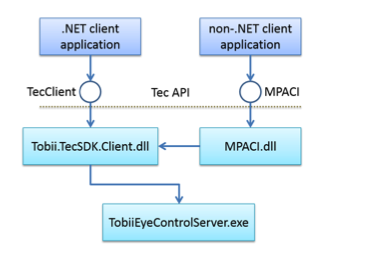
\includegraphics[width=100mm]{SoftwareArchitectureOverview}
\caption{Bilde som viser programvare arkitekturen til blikk programvaren}
\label{fig:overview}
\end{figure}


\subsection{TecClient}

TecClient støtter to GUI rammeverk; Windows Presentation Foundation (\gls{WPF}) og Windows Forms. 
 (kilde dokumentasjon).  Samhandling mellom applikasjonen og TecClienten skjer gjennom et konsept som de har valgt å kalle TecClients verktøykasse. De ulike verkøys klassene er presentert i figur \ref{fig:toolbox}. 

\begin{figure}[ht!]
\centering
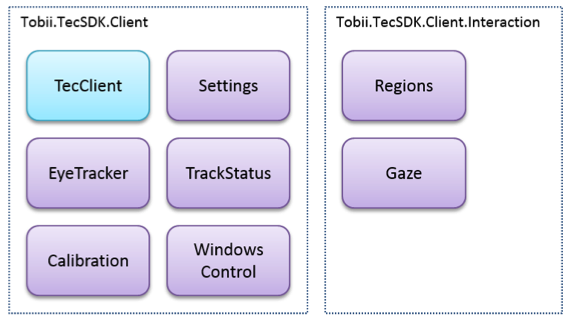
\includegraphics[width=100mm]{Toolbox}
\caption{Verktøy klassser som er tilgjengelige gjennom TecClient komponenten verktøyskasse}
\label{fig:toolbox}
\end{figure}


\subsubsection{EyeTracker}
Gir informasjon om den aktuelle øyesporingsenheten.

\subsubsection{Kalibrering}
Tilbyr tilgang til kalibrerings funksjonalitet og innstillinger som kan bli brukt for å kontroller hvordan kalibreringen er gjort.

\subsubsection{Settings}
Settings gir tilgang til bruker og klient innstillinger. Med mulighet til å hente nåværende bruker, alle bruker med funksjonalitet til å legge til og fjerne brukere og nåværende klient.

\subsubsection{Trackstatus}
Tilbyr metoder, egenskaper og hendelser for å kontrollere sporingsstatus vinduet. 


\subsubsection{Regions}
Tilbyr metoder, egenskaper og hendelser relatert til interaksjonsregioner. (1) Legge til og fjerne interaksjonsregioner, (2) hente informasjon om fokus og (3) søke etter interaksjonsregioner.

\subsubsection{Gaze}
Eksponerer blikkdata, både filtrert og ufiltrert. 
